% !TEX root = C:\Users\Jan\Documents\dev\Risk-Measurement-Framework\masterthesis_tex\masterthesis_main.tex

\section{Risk-Measurement-Framework concept and design}
\label{sec:conFrame}

In contrast to Schwerdtner et al. \cite{DBLP:journals/corr/abs-2011-04328}, the framework of this thesis concentrates on training, especially risk measurement before and during training of the ML model. The conceptual framework discusses and explains the design of the RMF. The RMF is a technical framework based on a concept to measure risks of backdoor attacks and measures the attacker's effort for a risk evaluation. \\ Referencing on this thesis approach from Biggio et al. \cite{DBLP:conf/icml/BiggioNL12} a security analysis for machine learning is that the attacker knows the ML model and can use the data from the data distribution platform. It is assumed for the RMF that the attacker knows the training data. This is an unrealistic assumption, but in real-world scenarios the attacker could use a surrogate training set instead, from the same data distribution platform which the developers use \cite{DBLP:journals/ml/BarrenoNJT10}. This subsection goes to the research question \ref{itm:rq1} - How can ISO 27004 be used to measure risks in machine learning?

\subsection{Using the standards for the risk measurement}
\label{sec:standard}

After the explained measures and measurement development based on ISO 27004 in section \ref{sec:relWork}, the next step is to map requirements into the RMF. This discussion what parts of them can be fulfilled and which parts can not fulfilled. That should show which requirements are fulfilled before using the RMF and where to document and communicate the results of the RMF. \\ \\

\textbf{''Defining the measurement scope''} where the organizations capabilites and resources define the initial scope. It starts by decisions of the management and can not be fulfilled by the RMF because that is an individual process specific for an organization and stands not in relation with the risk measurement of this thesis. The part defining stakeholder can not be fulfilled by the RMF but in ''Developing measurement constructs'' it will be further discussed how to identify them.  \\ \\

\textbf{''Identifying an information need''} is about the identification of an information need. The first activity of identifying the processes and examination of the ISMS can not be fulfilled of the RMF. The information need prioritization criteria like risk treatment can be fulfilled by the general riks measurement of the framework because all results are shown as transparent as possible. The organization's capabilities and resources criteria is individual for the organization and can not be measured. The interest of stakeholders are individual and must be defined before using the RMF. The third activity can be fulfilled by showing all results of the risk measurement in a document. Based on the third activity the RMF gives a document as an output which template is shown in appendix \ref{sec:template}. The last acitivity is a process which can be fulfilled after using the RMF. \\ \\

\textbf{''Selecting the object of measurement and its attributes''} describe that objects and attributes are identified in the scope and context of an ISMS, the objects and attributes need to be related to ML metrics which are used to measure risks and calculate the final risk. Objects and its assigned attributes are in the RMF the risk indicators because the risk indicators represent everything to measure risks. In order to assign the terms of objects, attributes, and base measures to the RMF, all risk indicators are assigned to these standard terms.

\begin{figure}[ht!]
  \centering
  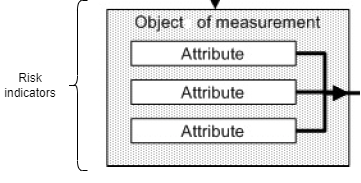
\includegraphics[width=10cm]{pictures/relation_risk_ind.png}
  \caption{Relation between the objects, attributes and the risk indicators adapted from \cite{ISO_27004_2009}}
  \label{fig:relation_risk_ind}
\end{figure}

As figure \ref{fig:relation_risk_ind} show adapted from \cite{ISO_27004_2009} the risk indicators are represented by objects and attributes in the ISO 27004 \cite{ISO_27004_2009} standard.
The terms of the standard thus enable a better classification and relationship of the terms assigned to the risk indicators. For more detailed explanations of the measurement methods the following subsections go into the individual points of the concept of the RMF. In order of this requirement attributes identify the type of measurement methods to obtain values which are assigned to the base measures. To fulfill the relation between the measurement methods that are selected through the attributes, there is a need to relate the attributes with a measurement method. \\ \\

\textbf{''Developing measurement constructs''} is about to define a measure selection, measurement method, measurement function, the analytical model, indicators, decision criteria, and stakeholders. Starting by identify a measure selection the following example criteria should help: facilitation for data collection, facilitation for interpretation, and measures to calculate costs of analysing, and collecting the data. The data collection can be done through the ML metrics for an attack. All of the collected data should be used for interpretation for the attack and the attacker's effort. Specificlly on poisoning attacks the training data must be analyzed and any information can be used to calculate the costs of analysing. It is complicated to find poisons because the modifications are small in images. The success depends on the patch size and the attacks on an image are highly specified \cite{DBLP:conf/icml/SchwarzschildGG21}. That could make the data collection harder and a final measure selection can be set up after the implementation of the RMF in the section \ref{sec:evaluation}. Therefore it is clearer to define the risk indicators as the measure selection. \\ The measurement method will be used to quantify the measurement object by transforming the attributes into the value that is assigned to the base measure. Measurement Methods can be subjective or objective. The objective measurement method measures based on the attack object. The high-level attributes which reflect the measurement about the attacker are subjective because they are in context of
human judgment \cite{DBLP:conf/crisis/DoynikovaNGK20}.

\begin{figure}[ht!]
  \centering
  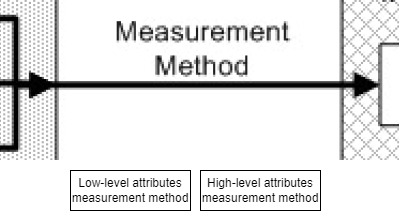
\includegraphics[width=10cm]{pictures/measurement_methods.png}
  \caption{The measurement method (right) send the collected data to the measurement method left (left). Both measurement method are executed at the second step of the measurement from ISO 27004 -  adapted from \cite{ISO_27004_2009}}
  \label{fig:measurement_methods}
\end{figure}

The outputs of the measurement methods need to be assigned to the base measures. Every base measure is an attributes from the objects but with
an assigned value. These base measures are used as the input for the measurement functions which are calculations to transform them into derived measures. That means the measurement functions are
calculations to transform the base measures into derived measured. In context to the risk measurement of the RMF this can be fulfilled for values which are not calculated already for example, the
accuracy is a value that is already a total value \cite{9783960101925} and do not need a further calculation with other results from the measurement method's output. \\ The analytical model is defined for each indicator by transforming values that are defined to a base or derived measure. These values should be transformed into a value that is assigned to an indicator. Indicators are assigend values that are assigned to aggregated values which in turn are assigned to derived measures. The analytical model creates outputs that are relevant for all stakeholders. This can not be fulfilled by the RMF because the stakeholders are not defined with the RMF. Since the relevant expenditures must be determined by the stakeholders, there must nevertheless be a selection of outputs that can be chosen by the stakeholders. \\ The values that are assigned to indicators and how they are presented describe ''Establishing data collection and analysis processes and tools''. Decision criteria are based on historical data, plans, and heuristics or calculated as statistical control or confidential limits. That process can not be fulfilled because the basis of the decision criteria is part which must be present before executing the RMF on a ML model. Stakeholders can be clients, reviewers for measurement, information owners or information communicators \cite{ISO_27004_2009} which can be identified as
Sharp et al. \cite{DBLP:conf/dexaw/SharpFG99} explain in their work.

\begin{figure}[ht!]
  \centering
  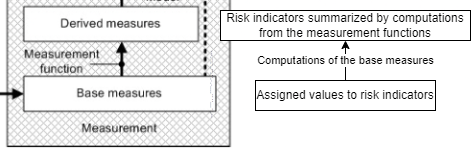
\includegraphics[width=10cm]{pictures/base_to_derived_measure.png}
  \caption{After the measurement methods are finished, the outputs are assigned to base measures and named as the risk indicators. A few risk indicators are calculated to derived measures - adapted from \cite{ISO_27004_2009}}
  \label{fig:base_to_derived_measure}
\end{figure}

Figure \ref{fig:base_to_derived_measure} shows the process after the measurment methods are finished and assigned their output to the base measures.\\ \\

\textbf{''Applying measurement constructs''} is a requirement that explains which information the measurement construct should contain. These information are the purpose of measurement, measurement objects, collected and used data, the data collection process and analysis, the process that reports measurement results, stakeholders and their roles and responsibilities, and a cycle to ensure the usefulness of measurements including the relation to the information needs \cite{ISO_27004_2009}. In context to the RMF the stakeholders and their roles and responsibilities, and the cycle to ensure the usefulness of measurements including the relation to the information needs can not be fulfilled. These information are not gathered from the RMF and it is not the goal of the RMF to collect these information. \\ \\

\textbf{''Establishing data collection and analysis processes and tools''} is the process of collect and analyse data to identify how the data is collected and stored with its necessary information of in the developed measurement results. This process can be fulfilled in all individual processes of the risk measurement in the RMF. The first acitivity how to store the collected data. The neccessary information are date, time, location of the data collection, information collector, information owner, any issues that happened during data collection, information for verification and measurement validation, and verify data against measure selection criteria and measurement constructs validation criteria. \\ The second acitivity can not be fulfilled by the RMF because it requires a communicator and stakeholders which analyse and interpret the data by human judgment. \\ \\

\textbf{''Establishing measurement implementation approach and documentation''} is the last requirement and describe the needed information from an implementation plan. This plan is not the basis of the implementation of the RMF because the process depends on organization's specifications and plans as a calendar which this thesis not using to design and implement the RMF. Instead of this implementation plan, subsection \ref{sec:final_design} show the final structure after which the RMF is implemented. \\ \\

In conclusion, with regard to the research question \ref{itm:rq1}, it can be stated that the requirements mentioned reflect only recommendations. That makes it possible to fulfill the requirements for security improvements in ML and confirms the hypothesis \ref{itm:h4} regarding to the requirements and procedures of ISO 27004.

\begin{table}[h!]
\centering
  \begin{tabular}{| c | p{10cm} |}
  \hline
  \rowcolor{lightgray} ISO 27004 term & Thesis mapping \\ [0.5ex]
  \hline
  Objects, Attributes & Represented by risk indicators \\
  \hline
  Measurement methods & Mapping low- and high-level attributes, measuring the low-level attributes \\
  \hline
  Measurement & Results from the measurement methods for evaluation to get the measurement results \\
  \hline
  Analytical model & \\
  \hline
  Indicators & \\
  \hline
  Decision criteria & \\
  \hline
  Base measures & Results from the measurement methods \\
  \hline
  Derived measure & \\
  \hline
  Measurement results & \\
  \hline
  \end{tabular}
\caption{Summarized mapping between the ISO 27004 and this thesis.}
\label{tab:iso_table}
\end{table}

\subsection{Risk indicators}
\label{sec:risk_indicators}

The RMF measure risks by so called risk indicators. Risk indicators are in context of ISO 27004 \cite{ISO_27004_2009} objects and attributes and represent the input data for the measurement methods. The input data are an object's attributes and assigned to the corresponding measurement method. Breier et al. \cite{DBLP:journals/corr/abs-2012-04884} in section \ref{sec:approaches} present
proposals that are the approach for the proposals of the risk indicators. These proposals are attack specificity, attack time, attacker's knowledge, and attacker's goal. The proposals have different subcategories which are visualized in figure \ref{fig:classifi_attacks_ml}. The attack specific proposals such as attack specificity, attack time are assigned to the low-level attributes. Attacker's knowledge and attacker's goal are assigned to the high-level attributes. These attributes are declared in the hypotheses \ref{itm:h2}, \ref{itm:h3}, \ref{itm:h5}, and \ref{itm:h6}.

\subsubsection*{Attributes and objects based on ISO 27004}

For the RMF the objects are separated into an object for the attack and an object for the attacker. To measure the risks on poisoning attacks and especially backdoor attacks, the RMF checks the training data for detecting outliers and checks where the data come from. \\ With reference to the approach already mentioned by Breier et al. \cite{DBLP:journals/corr/abs-2012-04884} the first four risk indicators for measuring risks are attack specificity, attack time, attacker's knowledge, and attacker's goal. Through their assignments to the low- and high-level attributes they are in turn assigned to the two objects. The attack time and attack specificity are attributes of the attack object and attacker's knowledge and also attacker's goal are attributes of the attacker object. Other than these attributes, there are also attributes which come from the ML model directly. These attributes are computational resources and TP, FP, TN, FN declared in the hypotheses \ref{itm:h1} and \ref{itm:h4}.

\begin{figure}[ht!]
  \centering
  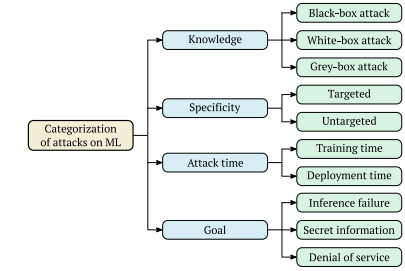
\includegraphics[width=10cm]{pictures/classifi_attacks_ml.png}
  \caption{Attack classifications on ML adapted from \cite{DBLP:journals/corr/abs-2012-04884}. The grey-box attack is not observed in this thesis}
  \label{fig:classifi_attacks_ml}
\end{figure}

\subsection{Measurement methods}

Risk measurement in the RMF starts after the identification of suitable objects and attributes with the selection of measurement methods according to the procedure of ISO 27004. As already mentioned in
the related work section \ref{sec:relWork}, there are different possibilities to execute poisoning attacks. At first, it is important to check where the training data come from. Xiao et al.
\cite{DBLP:conf/sp/XiaoLZX18} describe that training data can be polluted or mislabled when they come from external sources. Turner et al. \cite{turner2018clean} train a classifier with a small set of
clean input data where the input data are images from a trusted source that obtained or inspected the data. So, the more trustworthy a set of training data is, the lower the risk will be, and this
process can be transferred to the RMF. After the training data is checked for trustworthiness, the next part is to measure how large the extent of damage would be after a successful attack against the
ML model. The RMF needs to find out if the ML model is outsourced (Machine Learning as a Service, or MLaaS \cite{DBLP:journals/corr/abs-1708-06733}), if it is self-developed, or if the ML model comes
from an external resource and only has to be trained. For example, Google's Cloud Machine Learning Engine \cite{google_ai2022} allow's users to upload training data and a TensorFlow ML model to train it
in the cloud \cite{DBLP:journals/corr/abs-1708-06733}. \\ The other measurement method is used to find the attacker's effort. Finding the attacker's effort works according to the threat model of
Doynikova et al. \cite{DBLP:conf/crisis/DoynikovaNGK20} by analyzing the data from an attack. Therefore the measurement method to measure the extent of damage must be executed before measuring the
attacker's effort. The following sections \ref{sec:charac_backdoor}, \ref{sec:backdoor_types}, \ref{sec:ext_dmg}, \ref{sec:find_effort}, and \ref{sec:use_threat_model} explain the concept of the
measurement methods in the RMF.

\subsection{Characteristics of backdoor attacks}
\label{sec:charac_backdoor}

After discussing and evaluating the standards for the risk measurement in the RMF in section \ref{sec:standard}, this subsection explains which characteristics of backdoor attacks are measured in the
RMF. Biggio et al. \cite{DBLP:conf/icml/BiggioNL12} explain that poisoning attacks and therefore also backdoor attacks are causative attacks which means manipulations against training data is the focus of them. Further, Xiao et al. \cite{DBLP:conf/sp/XiaoLZX18} describe that training data can be polluted or mislabled when they come from external sources. Xiao et al. explain that poisoning attacks are not based on software vulnerabilities, which means that software bugs are not the execution point of backdoor attacks when implementing them into the RMF. This means the RMF measures conspicuities in the training data and measures the computational resources. Furthermore, the RMF measures before and after an attack to compare the differences between the original and manipulated ML model.

\subsection{Types of backdoor attacks}
\label{sec:backdoor_types}

The following backdoor attacks should represent what they can achieve when using them. Further, this subsection should show the main principles of the backdoor attacks that are used in the RMF.

\subsubsection*{Backdoor attack concepts}

\textit{PoisoningAttackBackdoor}, \textit{PoisoningAttackCleanLabelBackdoor}, and \textit{HiddenTriggerBackdoor} are the three backdoor attacks for this thesis. \\ \\
\textbf{PoisoningAttackBackdoor} Gu et al. \cite{DBLP:journals/corr/abs-1708-06733} explain \textit{PoisoningAttackBackdoor} which goal is to change original labels to a specific label on outsourced ML models. This happens by attacking a random small selection of the training set and apply a backdoor trigger into the input data. To be more precise, a backdoor attack works by adding a trigger in form of a pattern into some images in the training set, depending on the attack specificity (targeted or untargeted). Targeted means to poison specific images of a label that should trigger the backdoor if a pattern is on the images. Untargeted is an attack specificity through which images are random from a random label. This makes it difficult to detect the backdoor attack because the ML model's performance does not change in relation to the original performance. Backdoor attacks are powerful, because they take control over images that should be misclassified while the ML model is in test time \cite{turner2018clean}. In their work, Gu et al. show different backdoor attacks and perform a case study with a traffic sign detection attack on a neural network. The evaluated backdoors are a single pixel backdoor and a pattern backdoor. The single pixel backdoor increases the brightness of a pixel and the pattern backdoor adds a pattern of bright pixels in an image which is shown in Figure \ref{fig:backdoor_pattern}.

\begin{figure}[ht!]
  \centering
  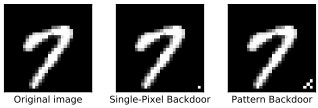
\includegraphics[width=10cm]{pictures/backdoor_pattern_bad_net.jpg}
  \caption{Backdoors in relation to the original image adapted from \cite{DBLP:journals/corr/abs-1708-06733}}
  \label{fig:backdoor_pattern}
\end{figure}

The implemented attacks from Gu et al. are a Single Target attack and an All-to-All attack where the training data is poisoned \cite{DBLP:conf/ccs/HuangJNRT11}. Single Target attacks use the single pixel backdoor by mapping a label from a digit (that is an image of the MNIST \cite{LeCun1995LearningAF} training set) $i$ as a digit $j$ on backdoored inputs. Figure \ref{fig:mapped_from_i_to_j} represents the classification error of the color-coded values where the row is $i$ and the column $j$.

\begin{figure}[ht!]
  \centering
  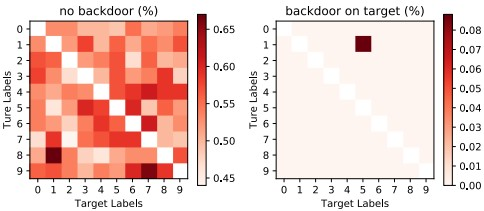
\includegraphics[width=10cm]{pictures/mapping_from_i_to_j.jpg}
  \caption{The left side shows the classification error (\%) of clean images with a Single Target attack for every instance. The right side shows the same but with backdoored images - adapted from \cite{DBLP:journals/corr/abs-1708-06733}}
  \label{fig:mapped_from_i_to_j}
\end{figure}

The attack strategy is a random pick of images from the training data and implements a poisoned version back to the training set. An All-to-All attack changes a digit label $i$ to $i + 1$. After testing the All-to-All attack, the original ML model has an error rate of 0.03\% while the ML model with the backdoored image has an average error of 0.56\%. \\ The case study is a traffic sign detection attack where the label of a stop sign is changed to a label of a speed limit sign. The backdoor of the image is either a yellow square, bomb image, or a sunflower image as the size of a post-it note on the stop sign. These backdoors are found at the bottom of the stop sign.

\begin{figure}[ht!]
  \centering
  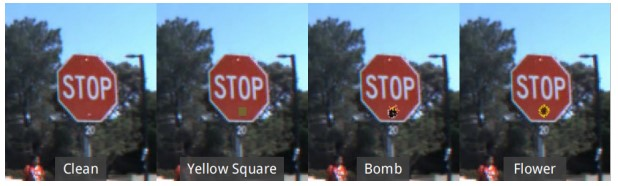
\includegraphics[width=10cm]{pictures/stop_sign.jpg}
  \caption{Stop sign as the clean version and with the three backdoors adapted from \cite{DBLP:journals/corr/abs-1708-06733}}
  \label{fig:stop_sign}
\end{figure}

The setup for the case study of Gu et al. bases on the Faster-RCNN \cite{DBLP:conf/nips/RenHGS15}. The Faster-RCNN takes an image as input data and the output data is a proposal as a set of rectangular objects where every rectangle has an objectness score.

\begin{figure}[ht!]
  \centering
  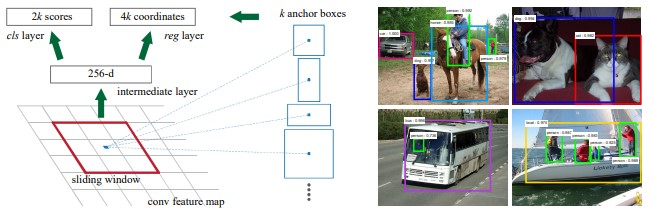
\includegraphics[width=10cm]{pictures/f_rcnn.jpg}
  \caption{The left side shows a region proposal network which represents the Faster-RCNN network and the right side shows an example of the detection adapted from \cite{DBLP:conf/nips/RenHGS15}}
  \label{fig:f_rcnn}
\end{figure}

The attack is a Single Target attack where the label of the stop sign image changes to a speed-limit label, and a random target attack where the stop sign is randomly changed to an incorrect label. The results show a successful pass of the validation tests and 90\% of the stop signs are missclassified as speed-limit signs. Gu et al. tested their ML model in a real-world attack by pasting a sticker on a stop sign near their office building. The ML model classified the stop sign with a 95\% confidence as a speed-limit sign. The ML model's accuracy is decreased on backdoors to 1.3\% which makes a misclassification to more than 98\%. This attack is now transferred to the RMF for risk measurement to check how much the accuracy is reduced. The more the accuracy for the classification of the poisoned images is decreased, the higher is the possible extent of damage which increases the risk. \\ \\
\textbf{PoisoningAttackCleanLabelBackdoor} In their work, Turner et al. \cite{turner2018clean} explain \textit{PoisoningAttackCleanLabelBackdoor} attacks in direct comparison to Gu et al. \textit{PoisoningAttackBackdoor}. Turner et al. show an approach for executing backdoor attacks by utilizing adversarial examples and Generative Adversarial Network (GAN)-generated data. The approach of Turner et al. is analyzing the effectiveness of the attack of Gu et al. while a simple technique is applied for data filtering. Data filtering is a technique to find poisoned data by comparing the used training data with trusted training data. Turner et al. discovered that the poisoned inputs are outliers and are clearly wrong from the human inspection side. The attack would be ineffective if it would rely solely on poisoned inputs which are labeled correctly and evade such filtering. At this point Turner et al. created an approach that poisons inputs which appear plausible to humans. The inputs need small changes to make them harder while classifying them but the original label must still remain plausible. This transformation is performed by a GAN-based interpolation and adversarial bounded pertubations. GAN-based interpolation takes each input into the GAN latent space \cite{DBLP:conf/nips/GoodfellowPMXWOCB14} and then interpolate poisoned samples to an incorrect class. Adversarial bounded pertubations use an optimization method to maximize the loss of the pre-trained ML model on poisoned inputs while staying around the original input. The main focus of this attack are poisoned samples that still have poisoned labels. That is why the attack is called Clean Label attack which is originally from \cite{DBLP:journals/corr/abs-1804-00792} in context of targeted poisoning attacks. Figure \ref{fig:poisoned_clean_label} shows an example airplane with different poisoned samples. The experiments base on the same patterns with a small black-and-white square in the bottom-right corner of the poisoned images as Gu et al. use in their work. The classifier is trained with the poisoned data and the test data are not labeled. The training dataset for the experiments
is the CIFAR-10 dataset \cite{Krizhevsky2009LearningML}. The ML model is a trained Wasserstein GAN \cite{DBLP:journals/corr/ArjovskyCB17}, \cite{DBLP:conf/nips/GulrajaniAADC17}. A GAN is strategy for training data where a game is defined between two competing networks. It contains a generator network and maps a noise source into the input space. A second network is the discriminator network which receives a generated sample or true data sample and then it must distinguish between those two samples. The Wasserstein GAN is using the Earth-Mover distance which is also called Wasserstein-1. For
further explanation of the mathematical structure, please see \cite{DBLP:journals/corr/GulrajaniAADC17}.

\begin{figure}[ht!]
  \centering
  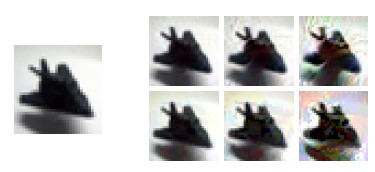
\includegraphics[width=10cm]{pictures/poisoned_clean_label.jpg}
  \caption{Difference between an original image and the conversion into adversarial examples with different pertubations adapted from \cite{turner2018clean}}
  \label{fig:poisoned_clean_label}
\end{figure}

\textbf{HiddenTriggerBackdoor} The last backdoor attack from Saha et al. \cite{DBLP:journals/corr/abs-1910-00033} is the \textit{HiddenTriggerBackdoor} which goal is to let poisoned data look natural with correct labels. This backdoor attack uses a threat model defined from Gu et al. \cite{DBLP:journals/corr/abs-1708-06733}. In this threat model, the attacker provides poisoned training data to a victim that uses it with a pre-trained ML model. The attacker uses a small image as a backdoor which changes the target label to a specific wrong label. This can be used for both attack specificity, targeted and untargeted. With this threat model it is possible to identify the poisoned data because as already explained in \textit{PoisoningAttackCleanLabelBackdoor}, the missclassified images change their label. Identifying the poisoned data in a training set can show how many images are poisoned to measure the extent of possible damage. Saha et al. propose a threat model inspired from Shafahi et al. \cite{DBLP:journals/corr/abs-1804-00792} and Sabour et al. \cite{DBLP:journals/corr/SabourCFF15} where the poisoned data are labeled correctly and the backdoor also remains not visible. This is done through optimization for poisoned images which pixel space is close to images from a target category while its feature space is close to source images that are patched with the backdoor. The next part is generalizing the attack for unseen source images which means that the trigger cannot be found during poisoning. Also the trigger should be placed at any random location. In order to implement this, during the optimization the poisoned images pushed close to a cluster of source images that are patched. Based on the work of Moosavi-Dezfooli et al. \cite{DBLP:conf/cvpr/Moosavi-Dezfooli17} about universal adversarial examples, Saha et al. minimized the value of loss at all source images and trigger locations. This is done by choosing a random trigger location and source images for each
iteration of optimization. Over every iteration a method optimizes randomly patched source images and assigns them to poisoned images closest to the feature space. Algorithm \ref{alg:poisoning_hidden} shows formally how the images are poisoned.

\begin{algorithm}
  \caption{Poisoning data algorithm adapted from \cite{DBLP:journals/corr/abs-1910-00033}}
  \label{alg:poisoning_hidden}
  \KwResult{$K$ poisoned images $z$ \\ 1. Sample $K$ random images \(t_{k}\) from the target category and initialize poisoned images \(z_{k}\) with them;}
  \While{\textit{loss} is \textit{large}}{
    2. Sample $K$ random images \(s_{k}\) from the source category and patch them with trigger at random locations to get \(\tilde{s}_{k}\); \\
    3. Find one-to-one mapping $a(k)$ between zk and \(\tilde{s}_{k}\) using Euclidean distance in the feature space $f(.)$; \\
    4. Perform one iteration of mini-batch projected gradient descent for the K-means clustering loss function;
  }
\end{algorithm}

\begin{figure}[ht!]
  \centering
  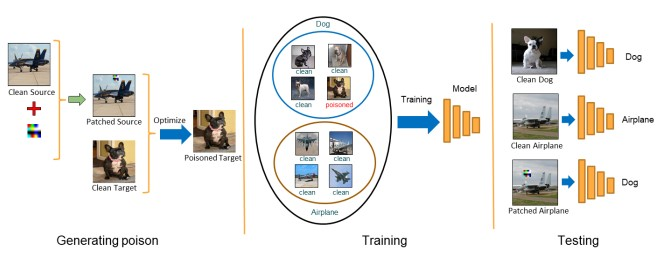
\includegraphics[width=10cm]{pictures/procedure_hidden_trigger.jpg}
  \caption{The left side visualize how an attacker generates a set of poisoned images. In the middle the visualization shows how the training data is extended by the poisoned data and then the victim trains the ML model. The right side visualize the test time. An attacker adds the backdoor trigger to images with the source category to manipulate the ML model without changing the label. This visualization is adapted from \cite{DBLP:journals/corr/abs-1910-00033}}
  \label{fig:procedure_hidden_trigger}
\end{figure}

\begin{figure}[ht!]
  \centering
  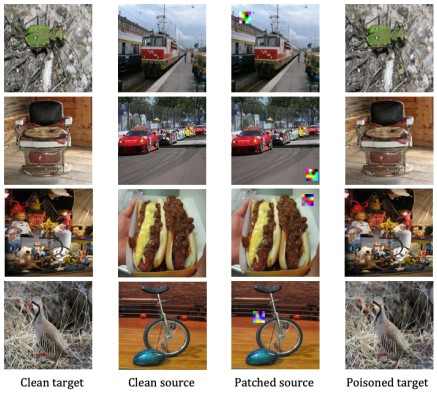
\includegraphics[width=11cm]{pictures/poisoned_hidden_trigger.jpg}
  \caption{The left side visualize how an attacker generates a set of poisoned images. In the middle the visualization shows how the training data is extended by the poisoned data and then the victim trains the ML model. The right side visualize the test time. An attacker adds the backdoor trigger to images with the source category to manipulate the ML model without changing the label. This visualization is adapted from \cite{DBLP:journals/corr/abs-1910-00033}.}
  \label{fig:poisoned_hidden_trigger}
\end{figure}

\subsection{Measure the extent of damage}
\label{sec:ext_dmg}

Based on the attacks, this subsection explains how the extent of damage is measured in the RMF. As the hypotheses \ref{itm:h4}, \ref{itm:h5}, and \ref{itm:h6} assume, the attack specificity, attack time, and the binary problem whith the positive and negative label are risk indicators. Based on \cite{DBLP:journals/corr/abs-1708-06733}, \cite{turner2018clean}, and \cite{DBLP:journals/corr/abs-1910-00033}, the accuracy metric of a ML model for a specific labeled image is a value that represents the success of a backdoor attack. Therefore, the accuracy is also a risk indicator to measure the extent of damage. All of these risk indicators are assigned with values before and after attack during training of the ML model. These data can be collected directly from the ML model which represents the low-level attributes in the threat model from Doynikova et al. \cite{DBLP:conf/crisis/DoynikovaNGK20}. To get these risk indicators assigned data the RMF needs a measurement method based on the low-
level attributes which concept describe subsection \ref{sec:use_threat_model}. After ML model training the RMF assigns the values of the risk indicators to the base measures which further process the values which subsection \ref{sec:derived_measures} describes.

\begin{figure}[ht!]
  \centering
  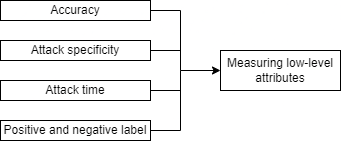
\includegraphics[width=9cm]{pictures/measure_damage.png}
  \caption{Risk indicators of the attack object in relation to the low-level attributes measurement method}
  \label{fig:measure_damage}
\end{figure}

\subsection{Measure the attacker's effort}
\label{sec:find_effort}

This subsection explains how the attacker's effort should be measured with the risk indicators proposed in Breier et al. \cite{DBLP:journals/corr/abs-2012-04884} and how the hypotheses \ref{itm:h2} and
\ref{itm:h3} should be proven. Further, this subsection explains how the risk indicator from the hypothesis \ref{itm:h1} should be proven. The risk indicators to find the attacker's effort are the
computational resources, the attacker's knowledge, and the attacker's goal. Starting with computational resources the RMF need to measure the computational resources that are mainly used to train a ML
model. The attacker's knowledge is divided into two possible knowledge levels. The first knowledge level are black-box attacks where the attacker has no information about the ML model. \\ In their
work, Papernot et al. \cite{DBLP:conf/ccs/PapernotMGJCS17} explain an attack strategy to misclassify a deep neural network by generated adversarial examples and get a misclassification rate of 84.24\%.
Papernot et al. assume that the attacker has no knowledge about the structure, parameters, and does not have access to any training set. The goal is to train a deep neural network with synthetic input
data and generated from the adversary. The output data are assigned labels from the targeted deep neural network and the adversary observe the output data. The input data are handwritten digits as
images and the output data are one of the digits. \\ The second knowledge level are white-box attacks where an attacker has nearly perfect knowledge about the ML model. Prinz and Flexer
\cite{DBLP:journals/corr/abs-2007-14714} present end-to-end adversarial attacks on classifications of music instruments. The training data are from the DCASE2019 Challenge \cite{DBLP:conf/dcase/
FonsecaPFES19}. In their work, Prinz and Flexer use four adversarial white-box attacks. Two attacks are untargeted
and called Fast Gradient Sign Method (FGSM) \cite{DBLP:journals/corr/GoodfellowSS14} and Projected Gradient Descent on the negative loss function (PGDn) \cite{DBLP:conf/iclr/MadryMSTV18}. The other two
targeted attacks are adaptions from the  Carlini and Wagner \cite{DBLP:conf/sp/Carlini018} method. The architecture is a convolutional neural network (CNN) as Figure \ref{fig:cnn_whitebox} shows.

\begin{figure}[ht!]
  \centering
  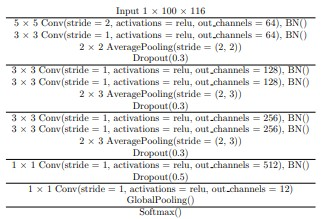
\includegraphics[width=8cm]{pictures/cnn_whitebox.jpg}
  \caption{The neworks contains $5x5$ and $3x3$ convolutional layers with the ReLU activation, batch normalisation, and average-pooling layers. The CNN uses dropout for regularisation and the final layer is a $1x1$ convolutional layer adapted from \cite{DBLP:journals/corr/abs-2007-14714}}
  \label{fig:cnn_whitebox}
\end{figure}

Prinz and Flexer \cite{DBLP:journals/corr/abs-2007-14714} and Papernot et al. \cite{DBLP:conf/ccs/PapernotMGJCS17} show both ways to attack ML models and in both works they used specific attacks for specific ML models. Both attacks bases on white-box or black-box attacks which shows that it is possible to find out if an attack is a black- or white-box attack. And when that is found out it should be possible measure the knowledge by pre-determined steps to execute the attack \cite{bsi_2013}. In the RMF, this is how the knowledge of the attacker is measured.

\begin{figure}[ht!]
  \centering
  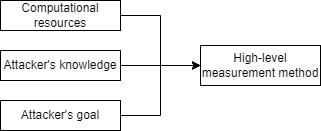
\includegraphics[width=9cm]{pictures/measure_effort.png}
  \caption{Risk indicators of the attacker object in relation to the high-level attributes measurement method}
  \label{fig:measure_effort}
\end{figure}

\subsection{Using the formal threat model}
\label{sec:use_threat_model}

To measure the extent of damage, subsection \ref{sec:ext_dmg} describe which risk indicators the RMF uses to get the corresponding values. As already explained in subsection \ref{sec:ext_dmg}, these values must be collected from the measurement method of the low-level attributes which explains this subsection. For this risk measurement the attacker's effort must also be evaluated how high or low the risk is for a ML model. The concept to measure the corresponding values that are assigned to the risk indicators describe subsection \ref{sec:find_effort} and is further explained here by the threat model. In this subsection the research questions \ref{itm:rq5}, \ref{itm:rq6} are addressed in more detail. In reference to the research question \ref{itm:rq8} this threat model is a
possible method for the RMF to measure risks which will be proved in section \ref{sec:evaluation}. As in section \ref{sec:threat} explained, the high- and low-level attributes have to be mapped to find the high-level attributes based on the low-level attributes.

\subsubsection*{The low-level attributes}

To find the attacker's effort there is a need to collect data which can be measured from every attack on a ML model. These data are classified and explained in section \ref{sec:threat}. Doynikova et al. \cite{DBLP:conf/crisis/DoynikovaNGK20} explained which data is required to meausre the low-level attributes. The low-level attributes that Doynikova et al. use in their work, event logs, network traffic, namely, and their source are possible to use in relation with the risk indicators. A possibilty for this is monitoring the values for the risk indicators with event logs, namely, and their source. The network can not be used because the RMF only measures an attack on a ML model without considering the network traffic because this thesis does not concentrate on MLaaS \cite{DBLP:conf/hci/HaraA21}.

\begin{enumerate}
  \item The first requirement is a dataset which contains information about the attack actions against a ML model. The information must be based on the skills, resources, intention, and motivation of the attacker.
  \item The second requirment for the dataset is that everything is marked in such a way that the analysis shows which actions the attacker performed. But this requirement is more about having multiple attackers or the analysis accross multiple attackers.
\end{enumerate}

The low-level attributes measure the extent of damage based on the collected data. Doynikova et al. also explain that the low-level attributes must be mapped to the high-level attributes to measure the attacker's effort. That means the data from the attack are collected only with the low-level attributes. Nevertheless the high-level attributes have delimited attributes which are not measured at the low-level attributes. This means the attributes must be evaluated in a separate measurement method afterwards.

\subsubsection*{The high-level attributes}

The high-level attributes show the attacker's effort based on the risk indicators attacker's knowledge, attacker's goal, and the computational resources used for the ML model. The four groups explained in subsection \ref{sec:threat} are placed in relation to the risk indicators. The first group includes characteristics such as skills, motivation and intention. The motivation and intention correspond to the attacker's goal. The skills are a characteristic that are represented in all risk indicators to find the attacker's effort. The second group characterizes the attacker's capabilities and show the characteristics as used resources. This group represents the computational resources risk indicator. This risk indicators measures which hardware an attacker needs to execute an attack. The third group incorporates the attacker in relation with the attacked system. This group includes the attacker's location, the privileges, his goals, the access and the attacker's knowledge. This part can be used for the RMF with the attacker's goals and attacker's knowledge. The attacker's location and privileges are not part of the risk measurement. The last group relates the attacker with the attack and the steps that are included to execute the attack. This group can be used to map the low- and high-level attributes what is explained next.

\subsubsection*{Mapping the low-level with the high-level attributes}
\label{sec:map_low_high}

For the measurment method it is important to measure the risks of an attack. That makes it possible to measure the risks of the attacker. Therefore the mapping must also lead the high- and low-level attributes to each other. This is designed in such a way that all risk indicators are measured while the ML model is trained and after it is attacked.

\subsection{Define measurement functions to calculate derived measures}
\label{sec:derived_measures}

Not every derived measure need to be calculated such as the accuracy.

\subsection{Define an analytical model for each indicator}

The indicators are the final results from the measurement and provide the transition to the measurement results. This is the last step before the measurement results.

\subsection{Develop measurement results by evaluating the risk measurement}

The measurment results term in table \ref{tab:iso_table} summarized how the results should be presented in the RMF. The implementation of the measurement results are possible through the decision criteria which are also defined in \cite{ISO_27004_2009}. The RMF show the results as visualized Python plots and calculated results. Both bases on the risk indicators.

\subsubsection*{Analyze the dataset for vulnerabilites}

In this subsection the concentration lays on the training data which are the attack point of poisoning and backdoor attacks \cite{DBLP:conf/eusipco/ArshadAQLY21}. The focus is on training data that come from an external source. Therefore it must be established that the sources are also trustworthy. A method to do this describe Turner et al. \cite{turner2018clean}. It must also be noted that external ML models do not poison images before training. \\
To check the trustworthiness of training data they can be compared with trusted training data. Another point is to train the model with direct input data that come from sources that are directly connected with the ML model \cite{DBLP:conf/sp/XiaoLZX18}. This can be checked by asking questions before executing the measurement with the RMF.

\subsubsection*{Logging the execution of the attack}

In the RMF every Python function send its process and output into a log-file except visualizations but it is logged on which data they are created.

\subsubsection*{Machine learning metrics for risk measurement}

With regard to poisoning attacks, the goal is to decrease the accuracy \cite{DBLP:conf/icml/BiggioNL12}, \cite{DBLP:journals/corr/abs-1708-06733}. But the RMF should also use the precision-recall, the F1-score and shows learning curve of the training process. That should make it possible to identify everything of the attacks. Also with regard to the attacker's effort could be every collected information of the ML model and the training data a possible value.

\subsubsection*{Vizualising the risk measurement}

To evaluate the risk measurement as good as possible all data should be visualized. This could show more possible insights from human judgment.

\begin{figure}[ht!]
  \centering
  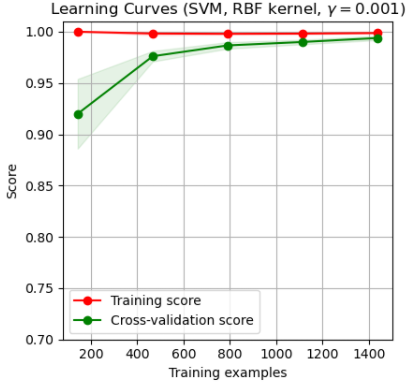
\includegraphics[width=8cm]{pictures/learning_curve_example.png}
  \caption{Learning curve example adapted from \url{https://scikit-learn.org/stable/auto_examples/model_selection/plot_learning_curve.html}}
  \label{fig:learning_curve_example}
\end{figure}

\subsubsection*{Calculate the risks}

The main calculation is $Risk = $ \textit{Extent of damage} $*$ \textit{Probability of occurence}. This calculation is intended to show how high the risk is for an ML model. Other calculations are to be displayed in detail as probabilities and stand in relation to the extent of damage or probability of occurance. For example, the composition of the extent of damage from the various risk indicators can be presented again in detail.

\subsection{The final design to implement the RMF}
\label{sec:final_design}

The last point \ref{itm:g} - ''Establishing measurement implementation approach and documentation'' of \ref{sec:standard} shows the needed information for an implementation plan. This subsection shows the final concept as a complete structure. At first a classifier check the trustworthiness of the training data by comparing the training data with trusted training data. To measure the extent of damage there need of an implementation of the low-level attributes. To get the attacker's effort another measurement method should represent the measurement of the high-level attributes. These two classes need to be mapped.

\begin{table}[h]
\centering
  \begin{tabular}{|c|p{10cm}|}
  \hline
  \multicolumn{2}{|c|}{Attack object} \\
  \hline
  \rowcolor{lightgray} Attributes & Description \\ [0.5ex]
  \hline
  Accuracy & The accuracy relates the number of data examples with true predicted labels to the number of all examined data examples \cite{9783960101925}. \\
  \hline
  TP, FP, TN, FN & \\
  \hline
  Attack specificity & The attack specificity can be targeted or untargeted \\
  \hline
  Attack time & The attack time differentiate between training and deployment time \\
  \hline
  \end{tabular}
\caption{ISO 27004 Object (attack)}
\label{tab:attack}
\end{table}

\begin{table}[h]
\centering
  \begin{tabular}{| c | p{10cm} |}
  \hline
  \multicolumn{2}{|c|}{Attacker object} \\
  \hline
  \rowcolor{lightgray} Attributes & Description \\ [0.5ex]
  \hline
  Attacker's goal & The attacker's goal can be a denial-of-service, doing an inference failure, or obtaining secret information \\
  \hline
  Attacker's knowledge & The knowledge of an attacker can be categoraized between white-, black-, or grey-box \\
  \hline
  Computational resources & The CPU, memory, GPU are the three parts which represent the used effort from the computer to attack and train a ML model. \\
  \hline
  \end{tabular}
\caption{ISO 27004 Object (attacker)}
\label{tab:attacker}
\end{table}
